\documentclass[tufte-handout]{standalone}
\usepackage{mathpazo} % Sets Palatino as the main font
\usepackage{tikz}
\usetikzlibrary{3d, angles, quotes, calc, backgrounds}
\usetikzlibrary{decorations.markings}

% my colors
\definecolor{darkslategray}{rgb}{0.18, 0.31, 0.31}
\definecolor{myorange}{rgb}{0.89804, 0.55686, 0.19608}

\begin{document}

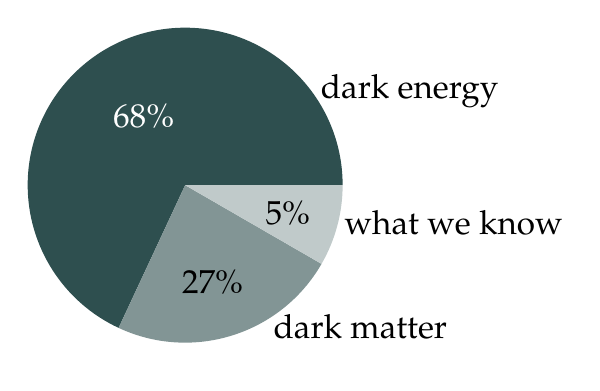
\begin{tikzpicture}
% Pie chart proportions
\begin{scope}
    % Draw the slices
    \fill[darkslategray] (0,0) -- (0:2) arc[start angle=0, end angle=245, radius=2] -- cycle; % Dark energy (~68%)
    \fill[darkslategray!60] (0,0) -- (245:2) arc[start angle=245, end angle=330, radius=2] -- cycle; % Dark matter (~27%)
    \fill[darkslategray!30] (0,0) -- (330:2) arc[start angle=330, end angle=360, radius=2] -- cycle; % What we know (~5%)

    % Add labels inside the pie chart
    \node[anchor=south west] at (150:1.2) {\large \textcolor{white}{$68\%$}};
    \node[anchor=east] at (305:1.5) {\large $27\%$};
    \node[anchor=north west] at (355:0.9) {\large $5\%$};

    
    % Add text labels for categories
    \node[anchor=west] at (1.6,1.2) {\large dark energy};
    \node[anchor=west] at (1,-1.8) {\large dark matter};
    \node[anchor=north west] at (1.9,-0.2) {\large what we know};
\end{scope}

\end{tikzpicture}

\end{document}
